\documentclass[twocolumn]{aastex61}
\usepackage{bm}
\usepackage{amsmath,amsfonts,amssymb}
\usepackage{color}
\usepackage{comment}

\newcommand\teff{T_{\rm eff}}
\newcommand\logg{\log{g}}
\newcommand\feh{[\rm{Fe}/\rm{H}]}

\newcommand{\project}[1]{\textsl{#1}}
\newcommand{\package}[1]{\texttt{#1}}
\newcommand{\acronym}[1]{{\small{#1}}}

\newcommand{\Gaia}{\project{Gaia}}
\newcommand{\gaia}{\project{gaia}}
\newcommand{\Galah}{\project{Galah}}
\newcommand{\GALAH}{\project{GALAH}}
\newcommand{\todo}[1]{\textcolor{red}{#1}}


\newcommand{\vect}[1]{\boldsymbol{\mathbf{#1}}}
\renewcommand{\vec}[1]{\vect{#1}}

\newcommand{\weight}{\pi}
\newcommand{\data}{\textbf{Y}}
\newcommand{\vecdata}{\vec\data}

\newcommand{\nextstep}{^\textrm{(t+1)}}
\newcommand{\thisstep}{^\textrm{(t)}}
\newcommand{\transpose}{^\intercal}
\newcommand{\eye}{\textbf{I}}

\newcommand{\factorloads}{\textbf{L}}
\newcommand{\factorscores}{\textbf{S}}
\newcommand{\specificvariance}{\vec{D}}

\newcommand{\scoremeans}{\vec\xi}
\newcommand{\scorecovs}{\vec\Omega}

\received{2018 XX XX}
\revised{2018 XX XX}
\accepted{2018 XX XX}

\newcommand{\vcpath}{vc.tex}

\IfFileExists{\vcpath}{\input{\vcpath}}{
	\newcommand{\giturl}{UNKNOWN}
	\newcommand{\gitslug}{UNKNOWN}
	\newcommand{\githash}{UNKNOWN}
	\newcommand{\gitdate}{UNKNOWN}
	\newcommand{\gitauthor}{UNKNOWN}
}



\submitjournal{AAS Journals}

\shorttitle{MCFA}
\shortauthors{Casey et al.}

\begin{document}

\title{MCFA on Galah}

\correspondingauthor{Andrew R. Casey}
\email{andrew.casey@monash.edu}

\author[0000-0003-0174-0564]{Andrew R. Casey}
\affiliation{School of Physics \& Astronomy, 
			 Monash University,
			 Wellington Rd, Clayton 3800, Victoria, Australia}
\affiliation{Faculty of Information Technology, 
			 Monash University, 
			 Wellington Rd, Clayton 3800, Victoria, Australia}
			 
\author{John Lattanzio}
\affiliation{School of Physics \& Astronomy, 
			 Monash University,
			 Wellington Rd, Clayton 3800, Victoria, Australia}

\author{Aldeida Aleti}
\affiliation{Faculty of Information Technology, 
			 Monash University, 
			 Wellington Rd, Clayton 3800, Victoria, Australia}

\author{David Dowe}
\affiliation{Faculty of Information Technology, 
			 Monash University, 
			 Wellington Rd, Clayton 3800, Victoria, Australia}

\author{the GALAH team}


\begin{abstract}
foo
\end{abstract}


\keywords{methods: statistical}

\section{Introduction} \label{sec:intro}

\section{Methods} \label{sec:methods}

% TODO: Is D a diagonal vector, or a matrix?! Make it consistent.

% Describe how we will attempt to define a generative model for the data, from the latent space.

In this work the data $\vecdata$ is a $n \times d$ matrix 
where $n$ is the number of stars and $d$ is the number of
chemical abundances measured for each star. We assume a
generative model for the data 
\begin{equation}
	\vecdata = \factorloads\factorscores + \vec{e}
	\label{eq:generative-model}
\end{equation}

\noindent{}where $\factorloads$ is a $p \times d$ matrix of factor
loads that is common to all data points, and the factor scores for
the $i$th data point
\begin{equation}
	\factorscores_i \sim \mathcal{N}(\vec\xi_k, \vec\Omega_k)
\end{equation}
\noindent{}are drawn from the $k$th multivariate  normal distribution.
The factor scores for all data points $\factorscores$ is then a 
\todo{$n \times p$} matrix.
 We assume $\vec{e} \sim \mathcal{N}\left(\vec{0}, \eye\specificvariance\right)$
is independent of the latent space, and $\specificvariance$ is a
diagonal matrix of $d$ entries. 

In this model each data point can be represented as being drawn
from a mixture of multivariate normal components, except the components
are \emph{clustered in the latent space} $\factorscores$ and projected
into the data space by the factor loads $\factorloads$. 
We assume that the latent space is lower dimensionality than the
data space (e.g., $p < d$).
Within the context of stellar abundances, the factor loads
$\factorloads$ can be thought of as the \emph{mean} yields
of nucleosynthetic
events (e.g., $s$-process yields from AGB stars), and the
factor scores are analogous to the relative counts of those 
nucleosynthetic events. The clustering in factor scores
achieves the same as a clustering procedure in data space,
except we simultaneously estimate the factor loads
(nucleosynthetic yields) that are common to all data points 
(stars). Within this framework a rare nucleosynthetic event
can still be described as a `common factor load' $\factorloads_i$, 
but its rarity would be represented by associated factor
scores being zero for most stars and thus have no contribution
to the observed abundances. The factor loads and factor scores 
cannot be expressly interpreted like this because they have no
physical meaning, but this description of relative yields and 
rates should help build intuition for the model parameters,
and provide an astrophysical context.


One benefit of using a mixture of common factor analysers is
for modelling stellar chemical abundances is the scaling with
computational cost. If we considered data sets of order $3\times10^7$
entries (e.g., 30 chemical abundances for $10^6$ stars) purely as a
clustering problem, then even the most efficient clustering
algorithms would incur a significant cumulative computational 
overhead by searching the parameter space for the number of
clusters, and the optimal model parameters given that number
of components. However, because the mixture of factor analyzers
approach assumes that there is a \emph{lower dimensional latent 
space} in which the data are clustered, and that clustering is 
projected into real space by common factor loads, the 
dimensionality of the clustering problem is reduced from 
$N \times D$ to $N \times J$. This reduces cost both through
faster execution of each E-M step, and on average fewer E-M steps
required to reach a specified convergence threshold.

From a statistical standpoint, the primary advantage to using
a mixture of factor analysers is that we can simultaneously
estimate latent factors (e.g., infer nucleosynthetic 
yields) and perform clustering (e.g., chemical tagging) 
within a statistically consistent framework. That is to say
that we have a generative model for the data that includes
analogues of nucleosynthetic yields and star formation,
and the parameters of this model can be estimated consistently
given some data.

Without loss of generality the density of the data $\vecdata$ can be modelled as
\begin{equation}
	f(\textbf{y}; \vec\Psi) = \sum_{k=1}^{K}\weight_{k}\phi(\textbf{y};\factorloads\scoremeans_k, \factorloads\scorecovs_k\factorloads\transpose + \eye\specificvariance)
\end{equation}
\noindent{}given $p$ common factor loadings and $K$ components
clustered in the latent (factor score) space. Here the parameter
vector
$\vec\Psi$ includes $\{\factorloads,\vec\pi,\scoremeans,\scorecovs,\specificvariance\}$, and $\phi(\textbf{y};\vec\mu, \vec\Sigma)$
describes the density of a multivariate gaussian distribution with
mean $\vec\mu$ and covariance matrix $\vec\Sigma$,
and $\weight_k$ describes the relative weighting of the $k$th
component in latent space and $\sum\weight_k = 1$.
The log likelihood is then given by
\begin{equation}
	\log\mathcal{L}(\vecdata|\vec\Psi) = \sum_{k=1}^{K}\log{f(\vecdata;\vec\Psi)} \quad .
\end{equation}


The model described by Equation~\ref{eq:generative-model} is indeterminate:
there is no unique solution for the factor loads $\factorloads$ and scores
$\factorscores$. However, an accurate estimate of the parameter vector $\vec\Psi$ can be obtained by the expectation-maximization algorithm \citep{EM}. 



\subsection{Initialisation}

We use the K-means++ algorithm to initially assign data points
randomly to $K$ clusters (in data space). This provides a so-called
hard initial association where each data point is wholly assigned
to a single component. Specifically we calculate the $n \times K$
responsibility matrix $\vec\tau$, where a entry of 1 indicates the
$n$th data point is associated with the $k$th cluster, and an
entry of 0 indicates no association such that
\begin{equation}
	\weight_k = \frac{1}{N}\sum_{n=1}^{N}\tau_{nk} \quad .
\end{equation}
We then chose 1,000
random data points and factorize that matrix using singular-value
decomposition. We take the principal $p$ eigenvectors as the 
initial guess for the factor loads $\factorloads$, and calculate
an initial estimate of the factor score means
\begin{equation}
	\scoremeans_k = \frac{1}{N}\sum_{n=1}^{N}\tau_{nk}\vecdata_{n}\factorloads
\end{equation}
\noindent{}and the covariance matrices of the clusters in latent space
\begin{equation}
	\scorecovs_k = \textrm{cov}{\left(\tau_{nk}\vecdata_{n}\right)} \quad .
\end{equation}


\subsection{Expectation-Maximization}

At the expectation step we evaluate the log likelihood
given the model parameters $\vec\Psi$, and we re-calculate the responsibility
matrix whose entries are the posterior probability
that the $n$th data point is associated to the $k$th component,
given the data $\vecdata$ and the current estimate of the 
parameter vector $\vec\Psi$:
\begin{equation}
	\tau_{nk} = \frac{\weight_k\phi(\vecdata_n;\factorloads\scoremeans_k, \factorloads\scorecovs_k\factorloads\transpose + \eye\specificvariance)}{\sum_{g=1}^{G}\weight_g\phi(\vecdata_n;\factorloads\scoremeans_g, \factorloads\scorecovs_g\factorloads\transpose + \eye\specificvariance)} \quad .
\end{equation}


% The complexity of SVD is O(n^3), and
% the complexity of K-means++ is O(log(k)). If we knew the complexity of
% k-means++ relative to N, then we would be able to make better decisions
% as to how to initialise: SVD first and then K-means in latent space?



% Discuss connection to PCA, FA, MFA.

% Include macros for \vec, \data, etc.
At the maximization step we update our estimates of the parameters,
conditioned on the data $y$ and the responsibility matrix $\vec\tau$.
Initially we update the relative weights $\vec\weight\nextstep$ given
the responsibility matrix $\vec\tau$
\begin{equation}
	\weight_k\nextstep = \frac{1}{N} \sum_{n=1}^{N}\tau_{nk} \quad .
	% Include proof.
\end{equation}


%\noindent{}In the equations that follow (Equation~\ref{eq:X} to \ref{eq:Y})
%when we refer to any value in $\{\factorloads,\vec\pi,\scoremeans,\scorecovs,\specificvariance\}$ for brevity we are referring to the current estimate of that
%parameter (e.g., $\factorloads\thisstep$). The updated estimates are marked as such
%(e.g., $\scoremeans\nextstep$). 

The updated estimates of the mean factor scores 
$\scoremeans\nextstep$ are given by
\begin{eqnarray}
	\scoremeans_{k}\nextstep = \scoremeans_{k}\thisstep + \frac{\vec{G}\transpose(\vecdata\transpose - \factorloads\thisstep\scoremeans_{k}\thisstep)\vec\tau_{k}}{N\weight_k\nextstep}
\end{eqnarray}
\noindent{}where:
\begin{eqnarray}
	\vec{W} &=& (\scorecovs_{k}\thisstep)^{-1}\eye \\
	\vec{V} &=& \left(\specificvariance\thisstep\right)^{-1} \\
	\vec{C} &=& (\vec{W} + (\factorloads\thisstep)\transpose\vec{V}\factorloads\thisstep)^{-1}\eye \\
	\vec{G} &=& \left[\vec{V} - \vec{V}\factorloads\thisstep\vec{C}\left(\vec{V}\factorloads\thisstep\right)\transpose\right]\factorloads\thisstep\scorecovs_k\thisstep \quad .
\end{eqnarray}

The covariance matrices of the components of factor scores $\scorecovs\nextstep$
are updated next,
\begin{equation}
	\scorecovs_k\nextstep = \left(\eye - \vec{G}\transpose\factorloads\thisstep\right)\scorecovs_k\thisstep + \frac{\vec{G}\transpose\vec{Z}\left(\vec{Z}\vec\tau_k\transpose\right)\transpose\vec{G}}{N\weight_k\nextstep}
\end{equation}
\noindent{}where
\begin{eqnarray}
	\vec{Z} &=& \vecdata\transpose - \factorloads\thisstep\scoremeans_k\thisstep \quad .
\end{eqnarray}

After some linear algebra, updated estimates of the common factor loads $\factorloads\thisstep$
can be found from
\begin{equation}
	\factorloads\nextstep = \factorloads_{1}\left(\factorloads_{2}^{-1}\eye\right)
\end{equation}
\noindent{}where:
\begin{eqnarray}
	\factorloads_1 &=& \sum_{k=1}^{K}\left[ \vec\tau_k\transpose\vecdata\left(\scoremeans_k\thisstep\right)\transpose + 
	\vec{G}\transpose\vec\tau_k\vec{Z}\transpose\vec{G}\right] \\
	%\left(\scoremeans_k\thisstep\vecdata\transpose\vec\tau_k\right)\transpose \left(\vec{G}\transpose\vec{Z}\vec\tau_k\transpose\vec{G}\right)\transpose\right]  \\
	\factorloads_2 &=& N\sum_{k=1}^{K}\left[\weight_k\nextstep\left(\scorecovs_k\nextstep + \scoremeans_k\nextstep\left(\scoremeans_k\nextstep\right)\transpose\right)\right]
\end{eqnarray}


Finally, the updated estimate of the specific variances $\specificvariance\nextstep$ is given
by
\begin{equation}
	\specificvariance\nextstep = \frac{1}{N}\left[\sum^{K}_{k=1}\vec\tau_k\transpose\left(\vecdata\odot\vecdata\right) - \sum_{j=1}^{J}\left(\factorloads\nextstep\factorloads_2\right)\odot\factorloads\nextstep\right]
\end{equation}

\noindent{}where $\odot$ denotes is the entrywise (Hadamard) product.


\section{Experiments} \label{sec:experiments}

\subsection{Toy model with generated data} \label{sec:experiment-toy-model}

We generated a data set with ${N = 100000}$ data points, each with
$D = 15$ dimensions, and assumed that those data are generated by
latent space of $J = 5$ ($J \times D$) factor loads, and there are $K = 20$
clusters in the latent space. The relative weights $\vec\weight$
are drawn from a multinomial distribution and the means of the clusters
in factor scores $\scoremeans$ are drawn from a standard normal
distribution. The covariance matrices in factor scores $\scorecovs$ are assumed to be diagonal matrices, where the non-zero entries are drawn from a gamma distribution $\scorecovs_{k,i,i} \sim \vec\Gamma\left(1\right)$. The variance in 
each dimension $\specificvariance$ are also drawn $\specificvariance \sim \vec\Gamma\left(1\right)$.
The $i$th data point (which belongs to the $k$th cluster) is then
generated by drawing $\factorscores_{i} \sim \mathcal{N}(\scoremeans_k,\scorecovs_k)$, projecting by the factor loads, and adding variance.

We fit this generated data using the expectation-maximization algorithm
as described in the previous Section. After 58 iterations
(and a serial processing time of 40 seconds) we
reached our convergence threshold: the log probability increased by
less than $10^{-5}$ with each iteration. For this experiment we specified
the number of latent factors $J$ and the number of clustering components
$K$ to include, but below we repeat this experiment where the number
of latent factors and clustering components is not known.

We show a corner plot of the data in Figure~\ref{fig:toy-model-data}.
In this figure we have over-plotted 100000 samples generated by the
estimated factor loads $\factorloads_\textrm{est}$ and the clustering in factor 
scores $\scoremeans_\textrm{est}$ and $\scorecovs_\textrm{est}$ (weighted by $\vec\weight_\textrm{est}$)
-- without adding variance $\specificvariance_\textrm{est}$ % Ref Factor load figure 
-- in order to illustrate that the
estimated model parameters can realistically generate the data.
The estimated latent space of factor scores is shown in 
Figure~\ref{fig:toy-model-latent-space} where the colours indicate the
most likely component that the data point is associated with.

Latent factor models are by definition indeterminate in that there are
multiple solutions of the parameter vector $\vec\Psi$ which provide
an identical data-generating process. This can be trivially shown by
the fact that the factors loads and scores can be rotated with some rotation
matrix $\textbf{R}$ and generate the exact same data. As a consequence,
we cannot strictly evaluate our model fitting procedure by comparing
how closely the inferred factor loads (or scores) match the true 
variables. This is further complicated by orientation and order
of the latent factors: even if the inferred factor loads were very close
to the true factor loads, they could be ordered differently, or have
their signs reversed. Given these issues, we evaluate the search as
being successful if the log probability given the estimated model
parameters is within convergence tolerance (or better) than the
log probability given the data and the true parameters.


% Despite not matching perfectly, it generates the data? property of uniqueness?
% Factor scores?
% Some metric about clustering performance against true values?


\begin{figure*}
	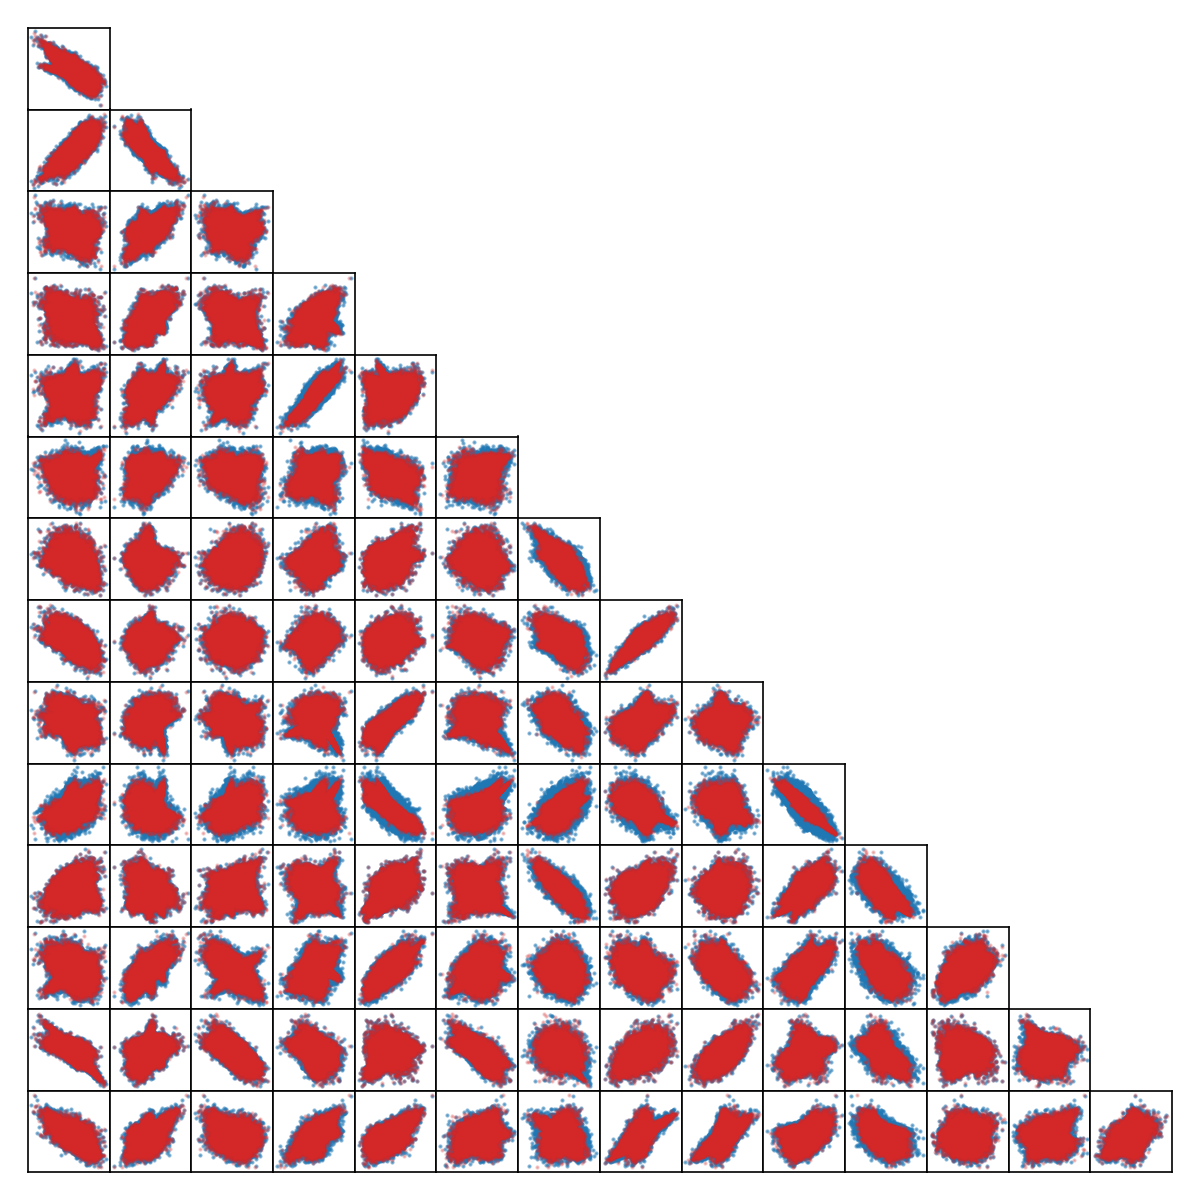
\includegraphics[width=1.0\textwidth]{experiments/toy-model-data.png}
    \caption{\todo{Caption}}
    \label{fig:toy-model-data}
\end{figure*}


\begin{figure*}
	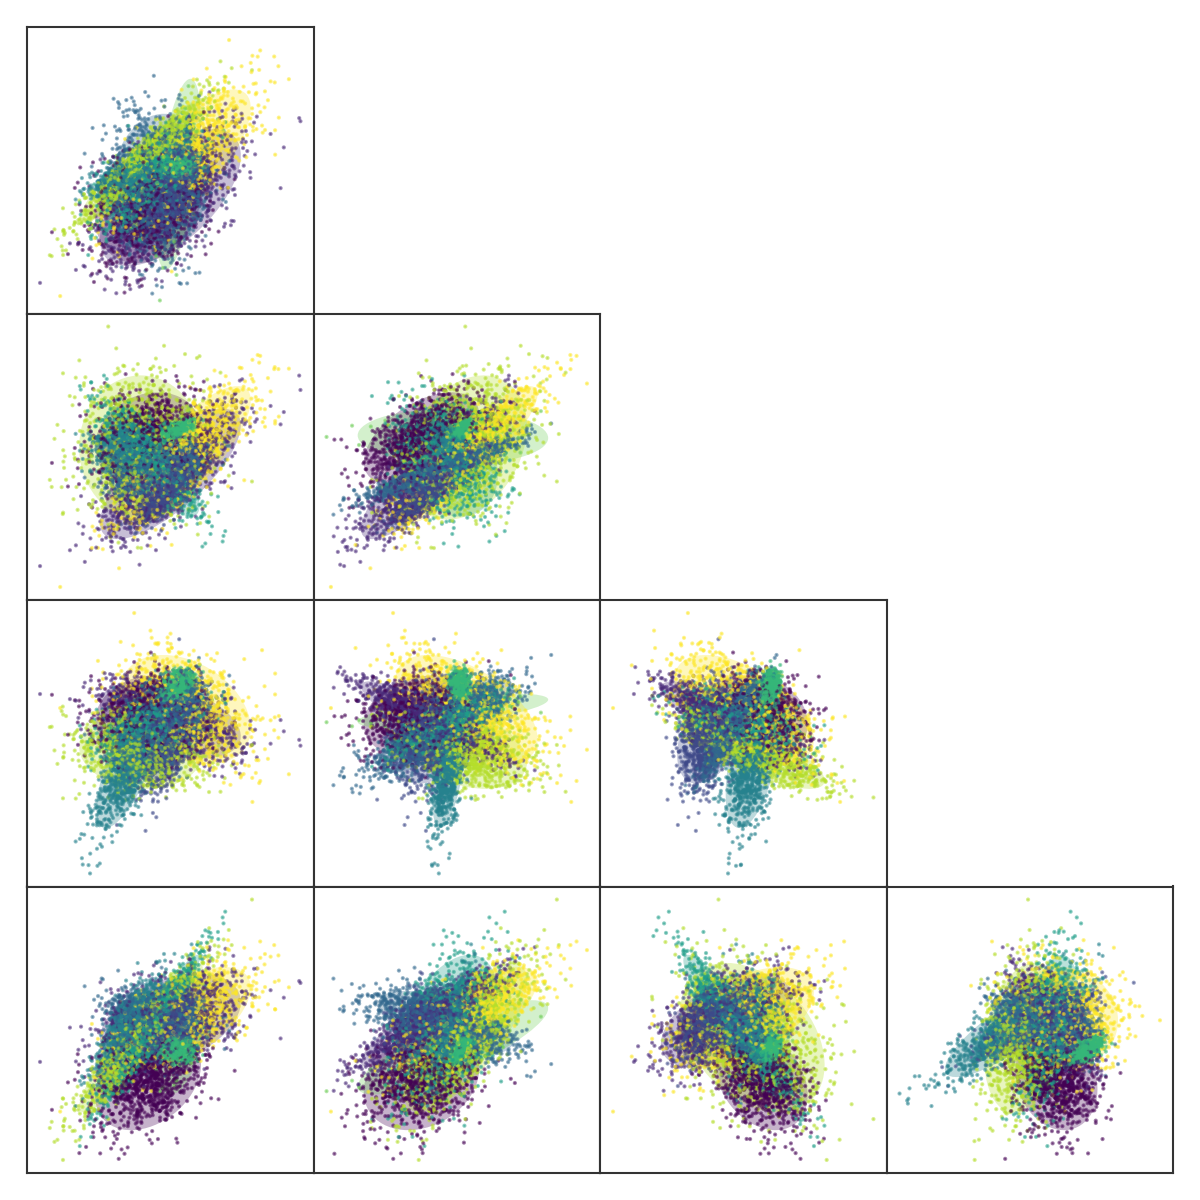
\includegraphics[width=1.0\textwidth]{experiments/toy-model-latent-space.png}
    \caption{\todo{Caption}}
    \label{fig:toy-model-latent-space}
\end{figure*}


% Search strategy for toy model.


% Figure: toy-model-factor-loads?
% Figure: toy-model-specific-variances?

\subsection{GALAH} \label{sec:experiment-galah}

The \Galah\ survey is a stellar spectroscopic survey of up to
$10^6$ stars. Up to 30 chemical abundances are expected to be measured
and reported in the final \Galah\ data release.
\todo{more about galah}

We use the second \Galah\ data release \citep{Buder:2018a} which
includes up to \todo{X} chemical abundances measured for \todo{Y}
stars. We selected stars with \texttt{flag\_cannon = 0} to exclude
stars where there is reason to suspect that the stellar parameters
(e.g., $\teff$, $\logg$) are unreliable, and as a result the 
detailed chemical abundances are untrustworthy. For this subset
we examined the measured abundances of \todo{X, etc} and
counted the number of stars with \texttt{flag\_x\_fe = 0}
for each abundance. This flag indicates that there is no known
reason to suspect that the measured chemical abundance is
unreliable. 

We sorted the elemental abundances by the number of stars
with reliable measurements, from highest to lowest. Starting
with Fe, we iterated over each element and counted the number
of stars with reliable measurements of that element and all
other elements earlier in the list. We illustrate this process
in Figure~\ref{fig:galah-abundance-flags}, where we show that
if we include the top 15 elemental abundances, we would have
\todo{X} stars with reliable measurements in all fifteen elements.
This is relevant to the approach we use here, as the method
described here requires no missing data.

% Where do we go down to?
% What elements do we add /remove.
\todo{Where do we go down to? What elements do we exclude?}
This leaves us with a sample of \todo{X} stars each with
reliable stellar parameters ($\teff$, $\logg$) and 
\todo{Y} (reliable) measured abundances: \todo{Mn, Fe}.
These elements are produced from multiple nucleosynthetic
pathways, including \todo{X}. 
It is this subsample that we will use for experiments
in chemical tagging.

\subsubsection{Search strategy} \label{sec:experiment-galah-search}

% Unknown number of latent factors and unknown number of latent scores



\section{Results} \label{sec:results}

\section{Discussion} \label{sec:discussion}

\section{Conclusions} \label{sec:conclusion}

\acknowledgements
A.~R.~C. is supported in part by Australian Research Council
Discovery Project DP160100637.
% Gaia acknowledgement?
% GALAH acknowledgement?

\software{
	\package{Astropy} \citep{astropy:v1,astropy:v2},
    \package{IPython} \citep{ipython},
    \package{matplotlib} \citep{mpl},
    \package{numpy} \citep{numpy},
    \package{scipy} \citep{scipy},
    \package{Stan} \citep{stan},
    \package{Jupyter Notebooks} \citep{jupyter-notebooks}
}    

\bibliographystyle{aasjournal}
\bibliography{mcfa}

\end{document}
